






\documentclass[a4paper]{article}

\usepackage{amsmath,amssymb,amsfonts}
\usepackage{graphicx,float,subfig}
\usepackage{booktabs}
\usepackage{fullpage}
\usepackage[colorlinks]{hyperref}
\usepackage{pdflscape}

\usepackage[font=small,labelfont=bf]{caption}

\renewcommand{\abstractname}{Aim}

\title{Estimation of Linear Attenuation Coefficient of Gamma Rays in Lead and Aluminum via Photoelectric and Compton Interaction}
\author{
    Oliver Kirkaptrick\footnote{s3725341@student.rmit.edu.au},
    Jackie Sholes\footnote{s3785864@student.rmit.edu.au},
    Anmolpreet Kaur Sodhi\footnote{s3838252@student.rmit.edu.au}
}


\begin{document}

\maketitle

\begin{abstract}
    The objective of this experiment is to determine the linear attenuation coefficient of gamma rays in lead and aluminum, and derive the mass absorption coefficient of these materials for gamma rays of varying energies. A gamma ray spectrometer is used to measure the decrease in the number of gamma rays detected as the thickness of a lead absorber is varied. The measurement of photoelectric or Compton interactions is used to calculate the attenuation coefficients. The spectrometer is calibrated using standard gamma-ray sources of known energies to ensure accurate measurement. The attenuation coefficients are then compared between the two materials, and the energy dependence of the coefficients is analyzed. The experimental results provide insights into the interaction of gamma rays with matter and have significant implications in a broad range of fields, such as radiation protection, nuclear medicine, and materials science.
\end{abstract}

\section{Relevant Theory}

As radiation passes through matter, some of that radiation will interact with the matter, giving the effect of reducing the total intensity of the radiation as it travels through the material. Similar to radioactive decay, we can model this reduction in intensity with an exponential relationship. Basically the exact same equation as well:

\begin{equation}
    I=I_{0}\mathrm{e}^{-\mu x}.
\end{equation}

Here, instead of decay rate $\gamma$ and time $t$, we have absorption coefficient $\mu$ and material thickness $x$. Similar to radioactive decay, where we have the concept of a half life, in attenuation of radiation by materials, we have the \textit{half value layer thickness}...which describes the thickness $x_{1/2}$ of material required such that $I=0.5I_{0}$. So, we let $I_{0}=1$ and thus $I=0.5$, and we can say

\begin{equation}
    I=I_{0}\mathrm{e}^{-\mu x}\Rightarrow 0.5 = \mathrm{e}^{-\mu x}\Rightarrow \frac{\ln{0.5}}{-\mu}=x_{1/2},
\end{equation}
or
\begin{equation}\label{eq:attenuation-coefficient}
    \mu=\frac{\ln{0.5}}{-x_{1/2}}.
\end{equation}
This half value layer thickness is then a convenient way to characterise materials with regards to their attenuation of radiation. If provided a half value layer thickness, we may then say for a given material which is $N$ ($\in\mathbb{R}^{+}$) times thicker than $x_{1/2}$, that the amount of attenuation is
\begin{equation}
    I=I_{0}\exp\left(-\mu\frac{N\ln0.5}{-\mu}\right)=I_{0}\exp\left(N\ln0.5\right)=I_{0}\frac{1}{2^{N}}.
\end{equation}
Another commonly quoted material property is the areal density of the material, which compensates for...material density. In all above equations, to get the areal density form, we replace $\mu$ with\footnote{sometimes high school algebra comes in handy}
\begin{equation}
    \frac{\mu}{\rho}\rho=\mu.
\end{equation}
An important property of a material which will affect its attenuation coefficient is the number of protons in the material. Materials with greater number of protons will tend to have higher attenuation coefficients due to their greater ability to interact with gamma rays via photoelectric, Compton, and pair production processes. This can be attributed to higher-Z materials providing more electrons to interact with the incoming gamma rays, leading to more scattering and absorption interactions, and thus faster attenuation.

Energy of incident gamma rays will also influence absorption coefficient. With increasing energy, gamma rays are more likely to pass through a given thickness of material without interacting. This will have the effect of requiring more material to accomplish equal attenuation, and thus reducing attenuation coefficient. Consider \eqref{eq:attenuation-coefficient}: as $x_{1/2}$ grows, it is clear that $\mu$ will become smaller---
\begin{equation}
    \mu\propto\frac{1}{x_{1/2}}.
\end{equation}
\section{Experiment Setup and Hardware}

The experiment utilized the following hardware, arranged as shown in~\autoref{fig:hardware-config}:
\begin{itemize}
\item NIM Bin and Power Supply
\item NaI(Tl) Crystal and Phototube Assembly
\item High Voltage Power Supply
\item Preamplifier
\item Amplifier
\item Oscilloscope
\item Ortec 928 Multi Channel Buffer, USB dual Port Memory cable, and PC with Maestro32 spectrum software for data analysis
\item $^{137}\mathrm{Cs}$, $^{22}\mathrm{Na}$, and $^{60}\mathrm{Co}$ gamma sources
\item Gain adjusted to xx to reach a maximum Oscilloscope reading of approximately 4 volts
\item Coarse gain set to xx, and fine gain set to 0.xx
\item Total gain set to xx
\end{itemize}

\begin{figure}[H]
\centering
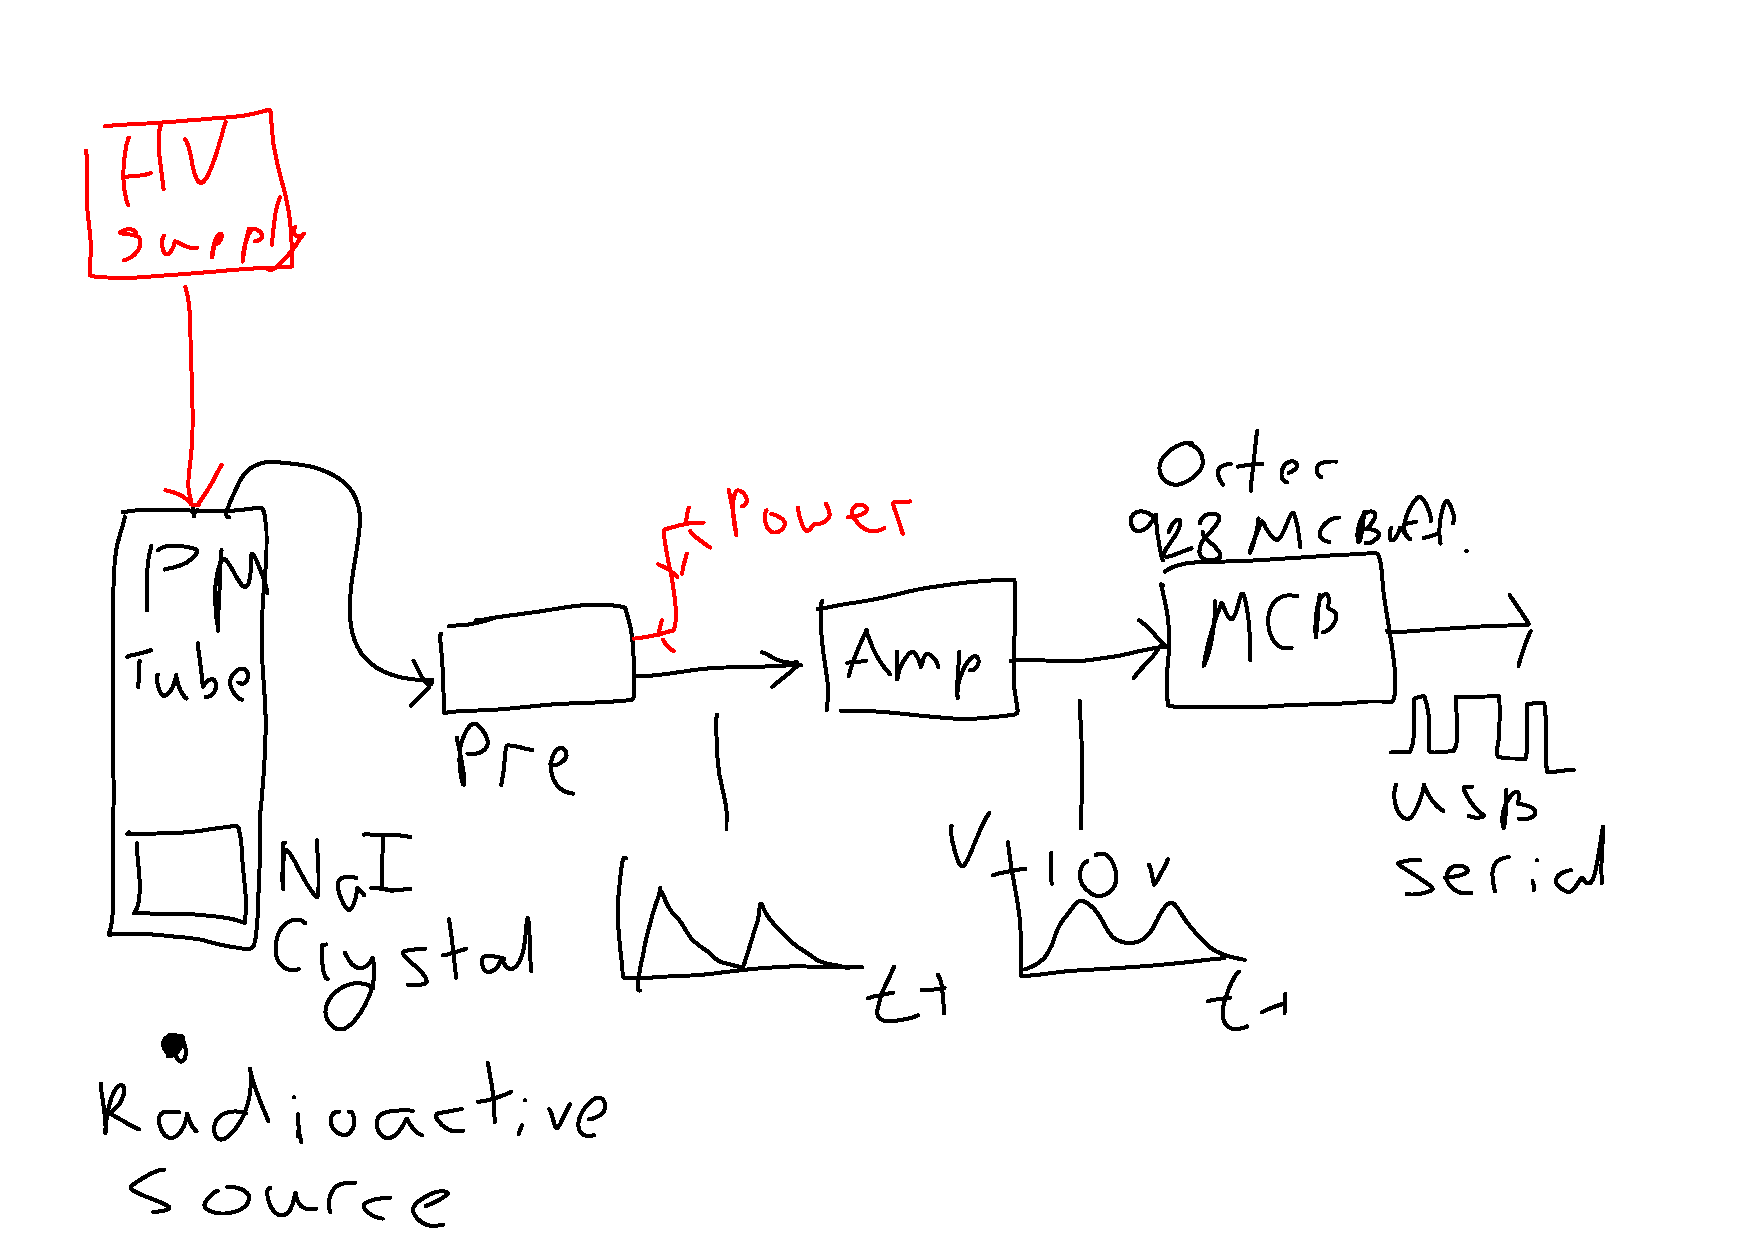
\includegraphics[width=0.6\textwidth]{figures/experiment-setup.pdf}
\caption{Base hardware configuration for calibration portion of the experiment--- PM Tube detects raw signals from a radioactive source placed approximately 2.5 cm away, which are then processed by the preamplifier and the amplifier. The signal peaks at around 10 V, and passes through the Multi-Channel Buffer for data analysis using Spectrum32 software on a computer.}
\label{fig:hardware-config}
\end{figure}

\subsection{Experimental Setup Procedures}

The setup procedures were carried out as follows:
\begin{enumerate}
\item Connect HV to the detector
\item Connect serial to preamp
\item Connect signal out of detector to 572A input
\item Connect T bridge out of uni to Oscilloscope and 928 MCB ADC in
\item Set initial scale from Oscilloscope to xx mV
\item Set initial pulse width to xx $\mu$s
\end{enumerate}
\section{Calibration Using $^{137}\mathrm{Cs}$, $^{22}\mathbf{Na}$, and $^{60}\mathrm{Co}$}
\subsection{Calibration}
\begin{itemize}
    \item initial height of photopeak was 1092 counts at live value of 10 seconds
    \item integration time increased to live value of 30 seconds
    \item 30 seconds produce 3107 counts
    \item ROI was set on 32 keV peak, and 662 keV peak
    \item 662 keV peak was identified as 662 keV, at bin 768.32, with FWHM of 43.84, library identified as cs 137
\end{itemize}

\subsection{Spectrum of $^{137}$Cs}
% \begin{figure}[H]
%     \centering
%     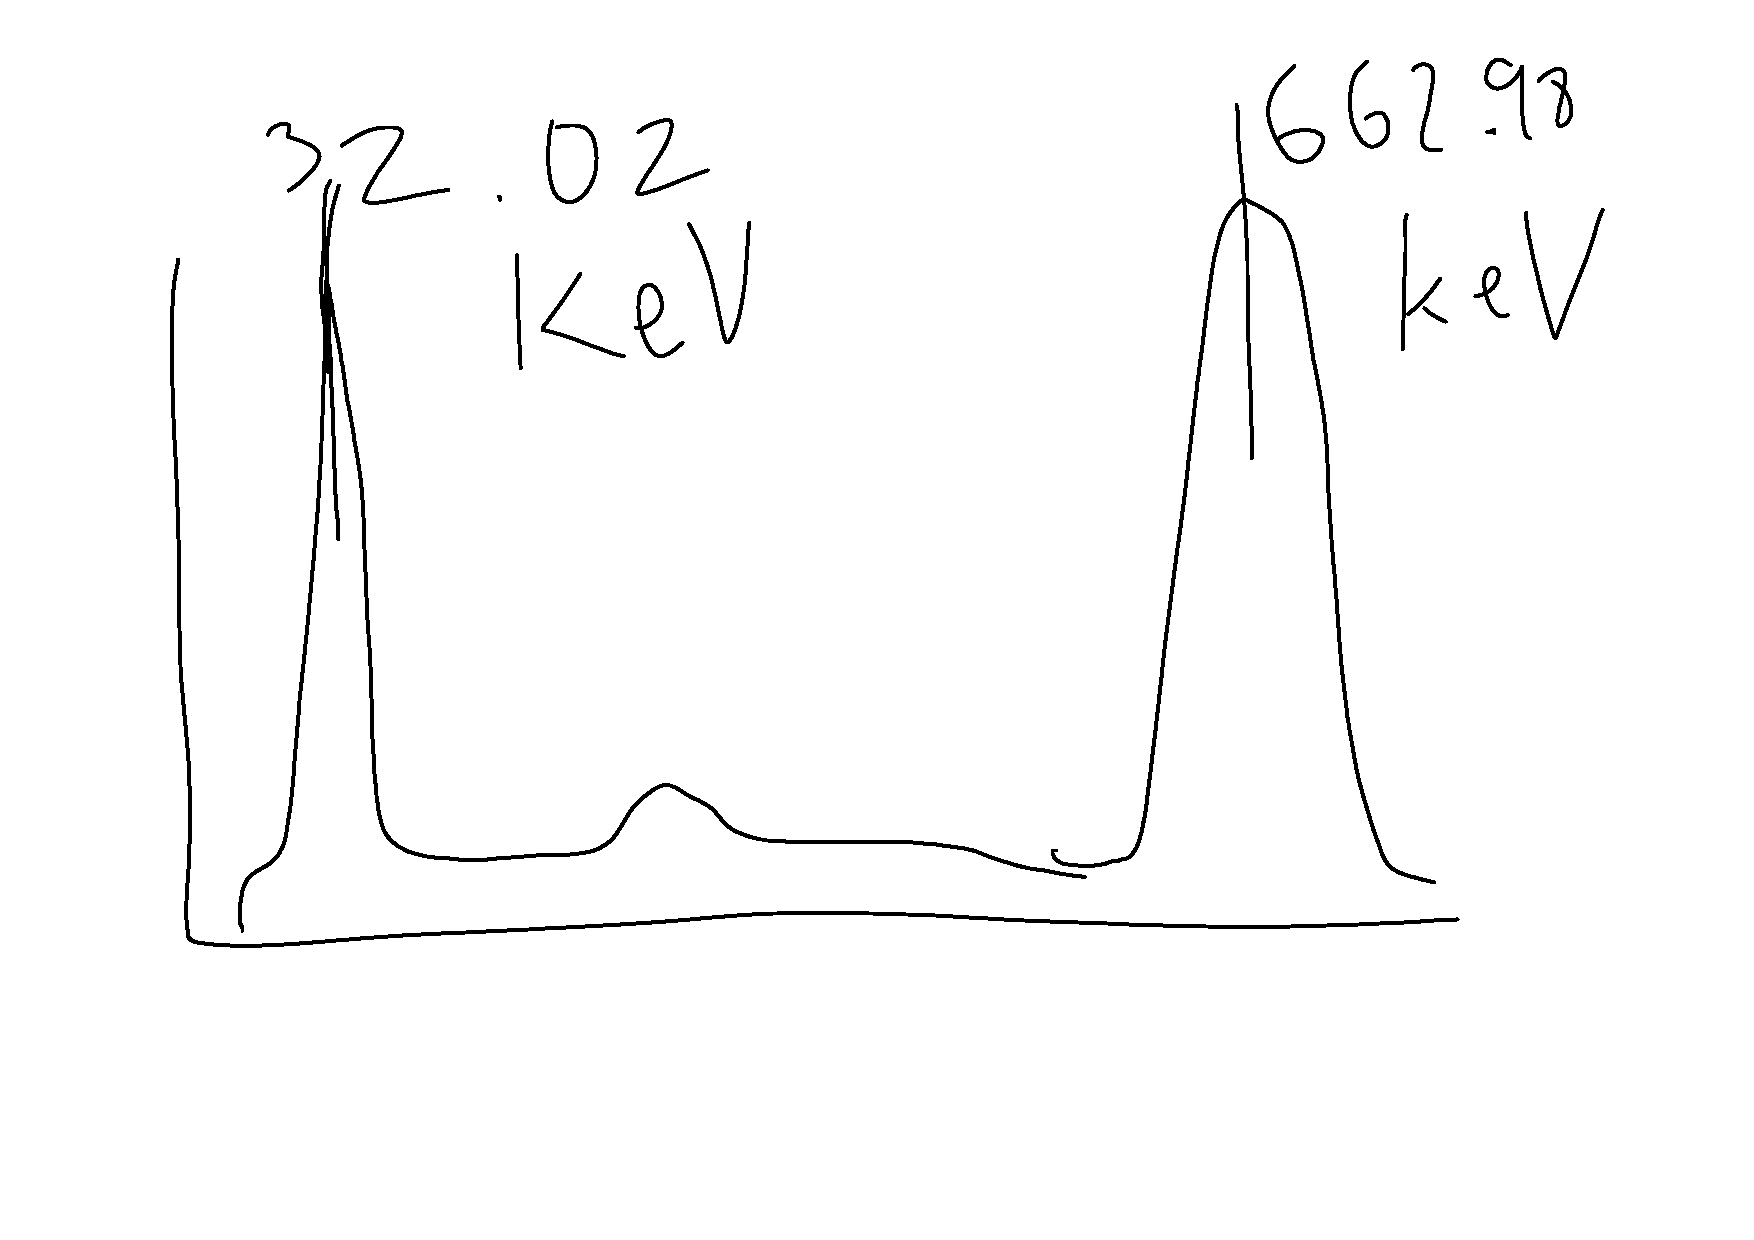
\includegraphics[width=0.75\textwidth]{figures/cesium_137_counts.pdf}
%     \caption{$^{137}$Cspectra of counts associated with varying energy bins. Two distinct peaks were identified, with the photo electric peak being centered (after calibration) at 662.98 keV, and the secondary peak presenting at 32.02 keV. A backscatter peak was recorded roughly between the two, however was not measured.}title
% \end{figure}
\begin{itemize}
    \item again, cesium was 2.5 cm away from face of detector
    \item 32 keV peak was identified as 32.01 keV, at bin 42.31, with FWHM as 7.21
    \item \verb|$MCA_CAL:-4.452449E+000 8.674188E-001 0.000000E+000 keV|
    \item \textbf{Data saved at: ./data/calibration\_spectrum\_cs.*}
\end{itemize}

\subsection{Spectrum of $^{22}$Na}
% \begin{figure}[H]
%     \centering
%     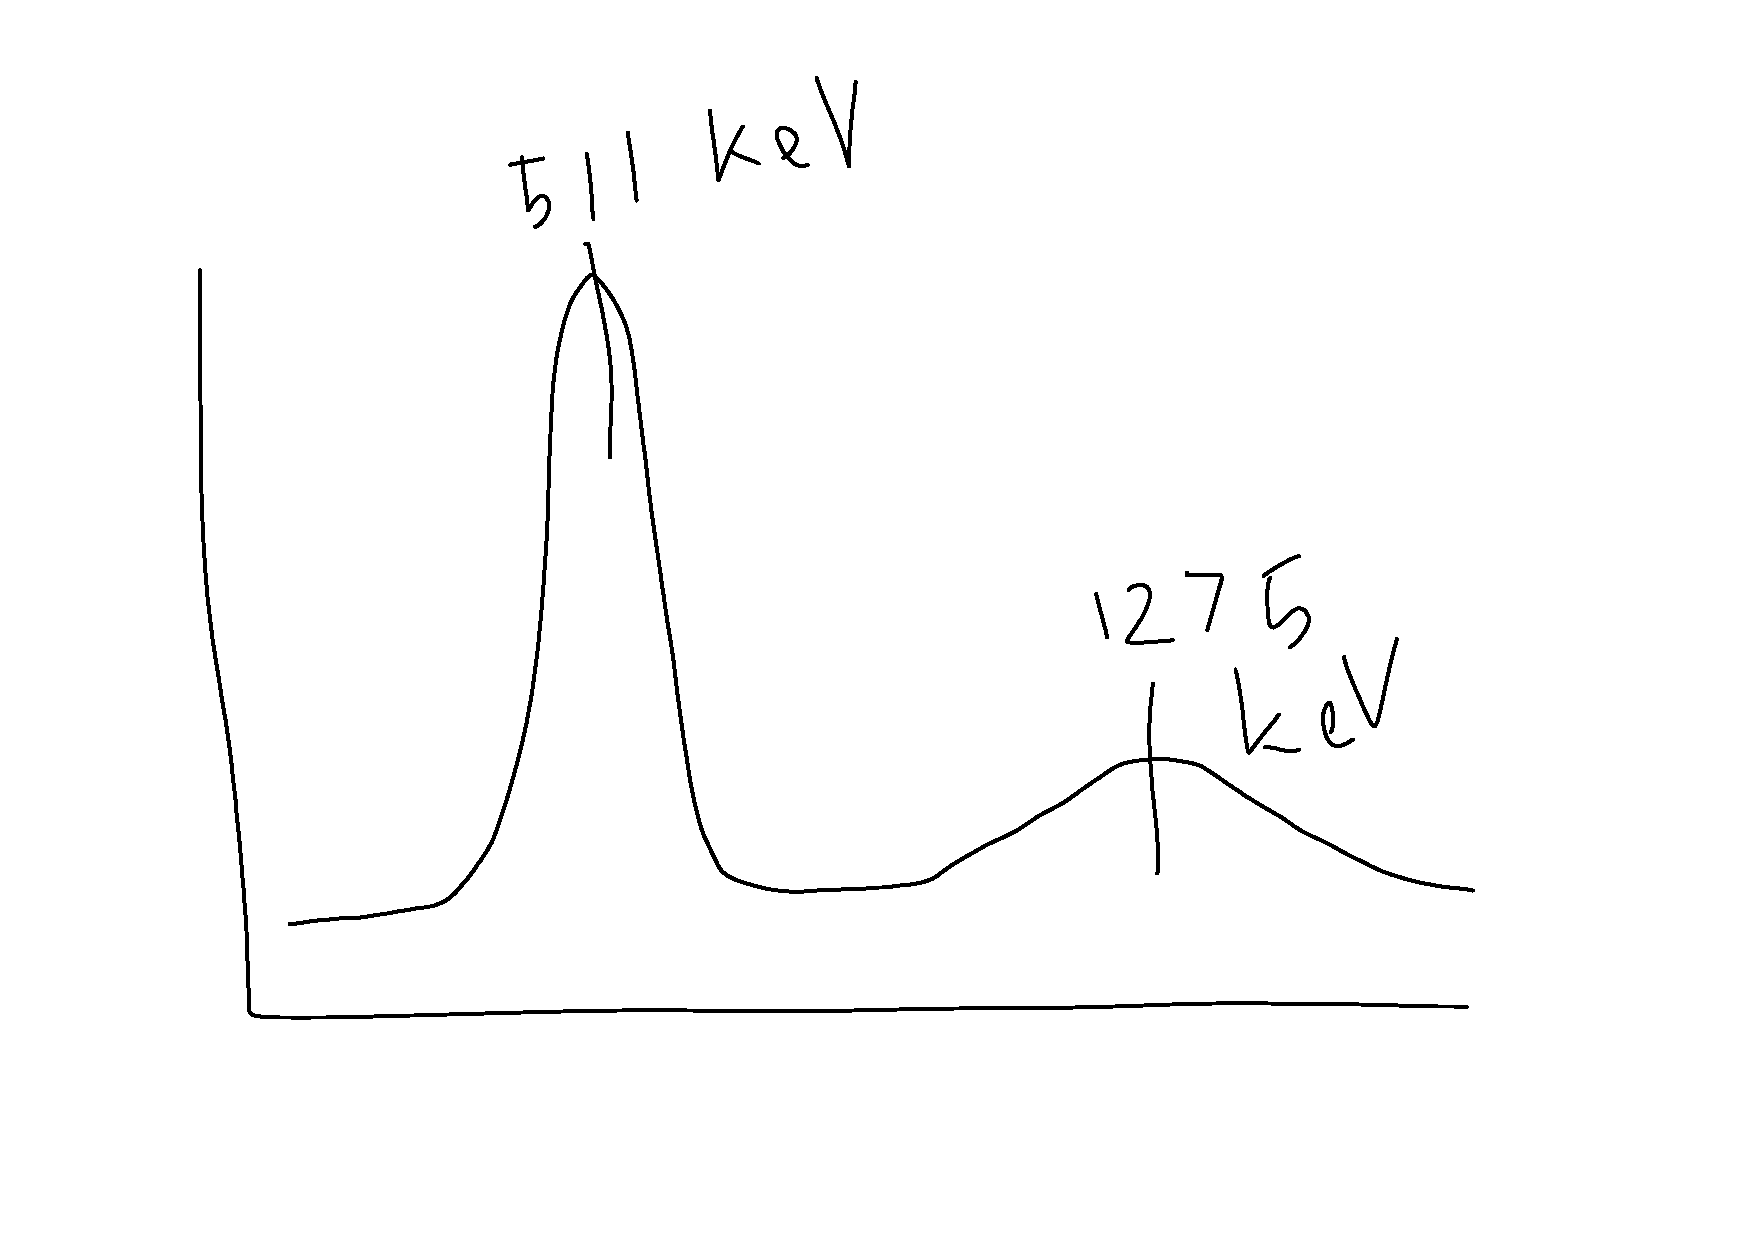
\includegraphics[width=0.75\textwidth]{figures/sodium_22_counts.pdf}
%     \caption{$^{22}$Na spectra of counts associated with varying energy bins. Two distinct peaks were identified, with no noticable smaller peaks, the photo electric peak being centered (after calibration) at 1275 keV, and the secondary peak presenting at 511 keV.}
% \end{figure}
\begin{itemize}
    \item again, sodium was place 2.5 cm away from face of detector
    \item first uncalibrated peak at 519 keV, bin at 604.34, should be 511 keV, FWHM was 37.65, suggested samarium for 521.28
    \item second uncalibrated peak at 1260.28 keV, at bin 1458.05, should be 1275, FWHM was 57.94
    \item calibration used 1260 peak
    \item after calibration first peak is at 511 keV, FWHM is 38.94, at bin 604.33, library suggests ytrium 88
    \item after calibration second peak is at 1274.54 keV, at bin 1458.04, FWHM was 59.96, library suggests sodium Na-22
    \item \verb|-2.948798E+001 8.943686E-001 0.000000E+000 keV|
    \item \textbf{Data saved at: ./data/calibration\_spectrum\_na.*}
\end{itemize}

\subsection{Spectrum of $^{60}$Co}
% \begin{figure}[H]
%     \centering
%     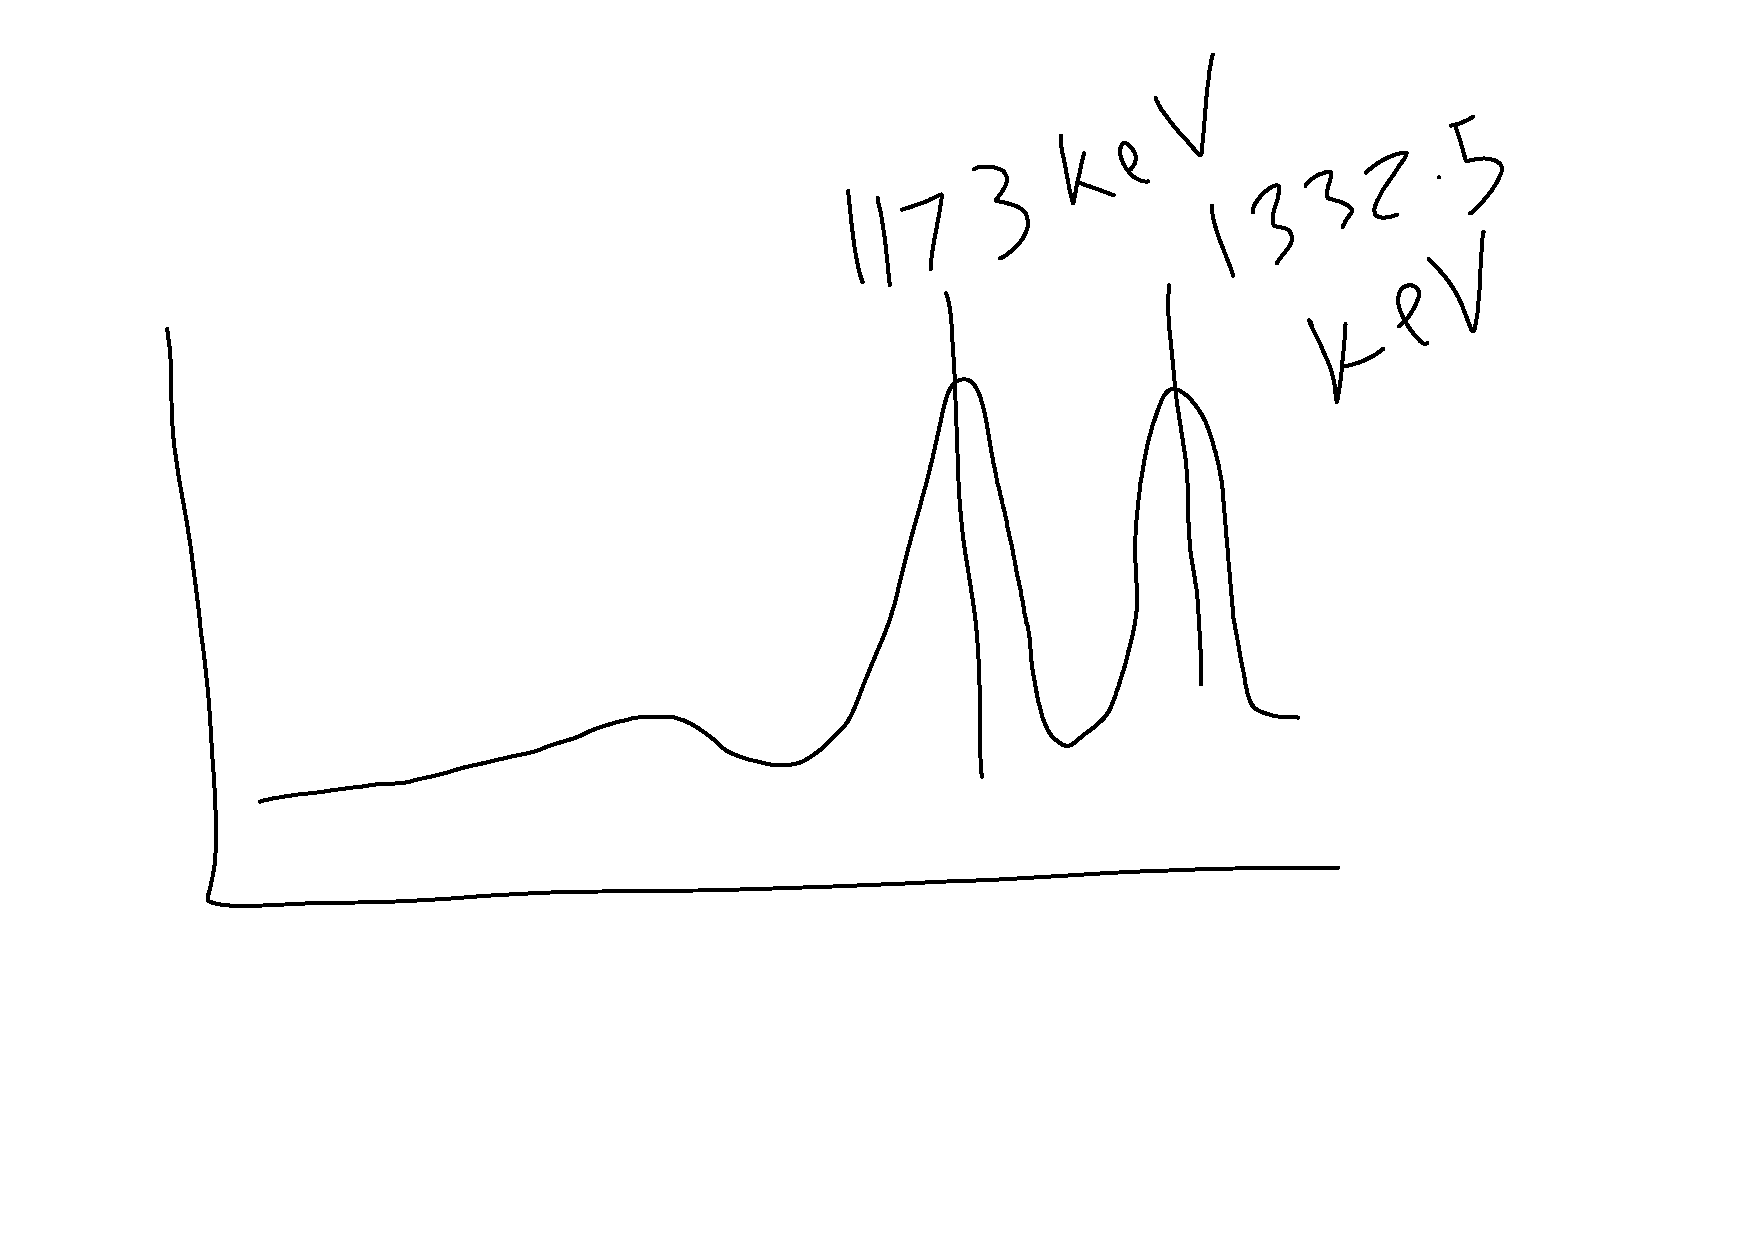
\includegraphics[width=0.75\textwidth]{figures/cobalt_60_counts.pdf}
%     \caption{$^{60}$Co spectra of counts associated with varying energy bins. Two distinct peaks were identified, with no noticable smaller peaks, the photo electric peak being centered (after calibration) at 1332.5 keV, and the secondary peak presenting at 1173 keV.}
% \end{figure}
\begin{itemize}
    \item again, cobalt was placed 2.5 cm away from face of detector
    \item reading on Oscilloscope was noticably higher than that of cesium and sodium
    \item size of peaks and number of counts on Maestro32 were significantly lower than those of cesium and sodium
    \item two peaks were identified, neighbouring one another
    \item first uncalibrated peak was at 1351 keV, at bin 1544.47, FWHM was 58.80, library suggests Iodine
    \item second uncalibrated peak was at 1192.70 keV, bin was 1366.54, FWHM was 50.96, library suggested Ta-182
    \item first photo peak calibrated to 1173.2 keV (did nothing), second to 1332.5 keV
    \item first peak calibrated to 1173.02 keV, bin at 1366.44, FWHM was 51.17, library suggested cobalt 60
    \item second peak calibrated to 1332.5, at bin 1544.57, FWHM was 64.25, library suggested cobalt 60
    \item \verb|-5.031831E+001 8.952744E-001 0.000000E+000 keV|
    \item \textbf{Data saved at: ./data/calibration\_spectrum\_na.*}
\end{itemize}

\subsection{Background}
% \begin{figure}[H]
%     \centering
%     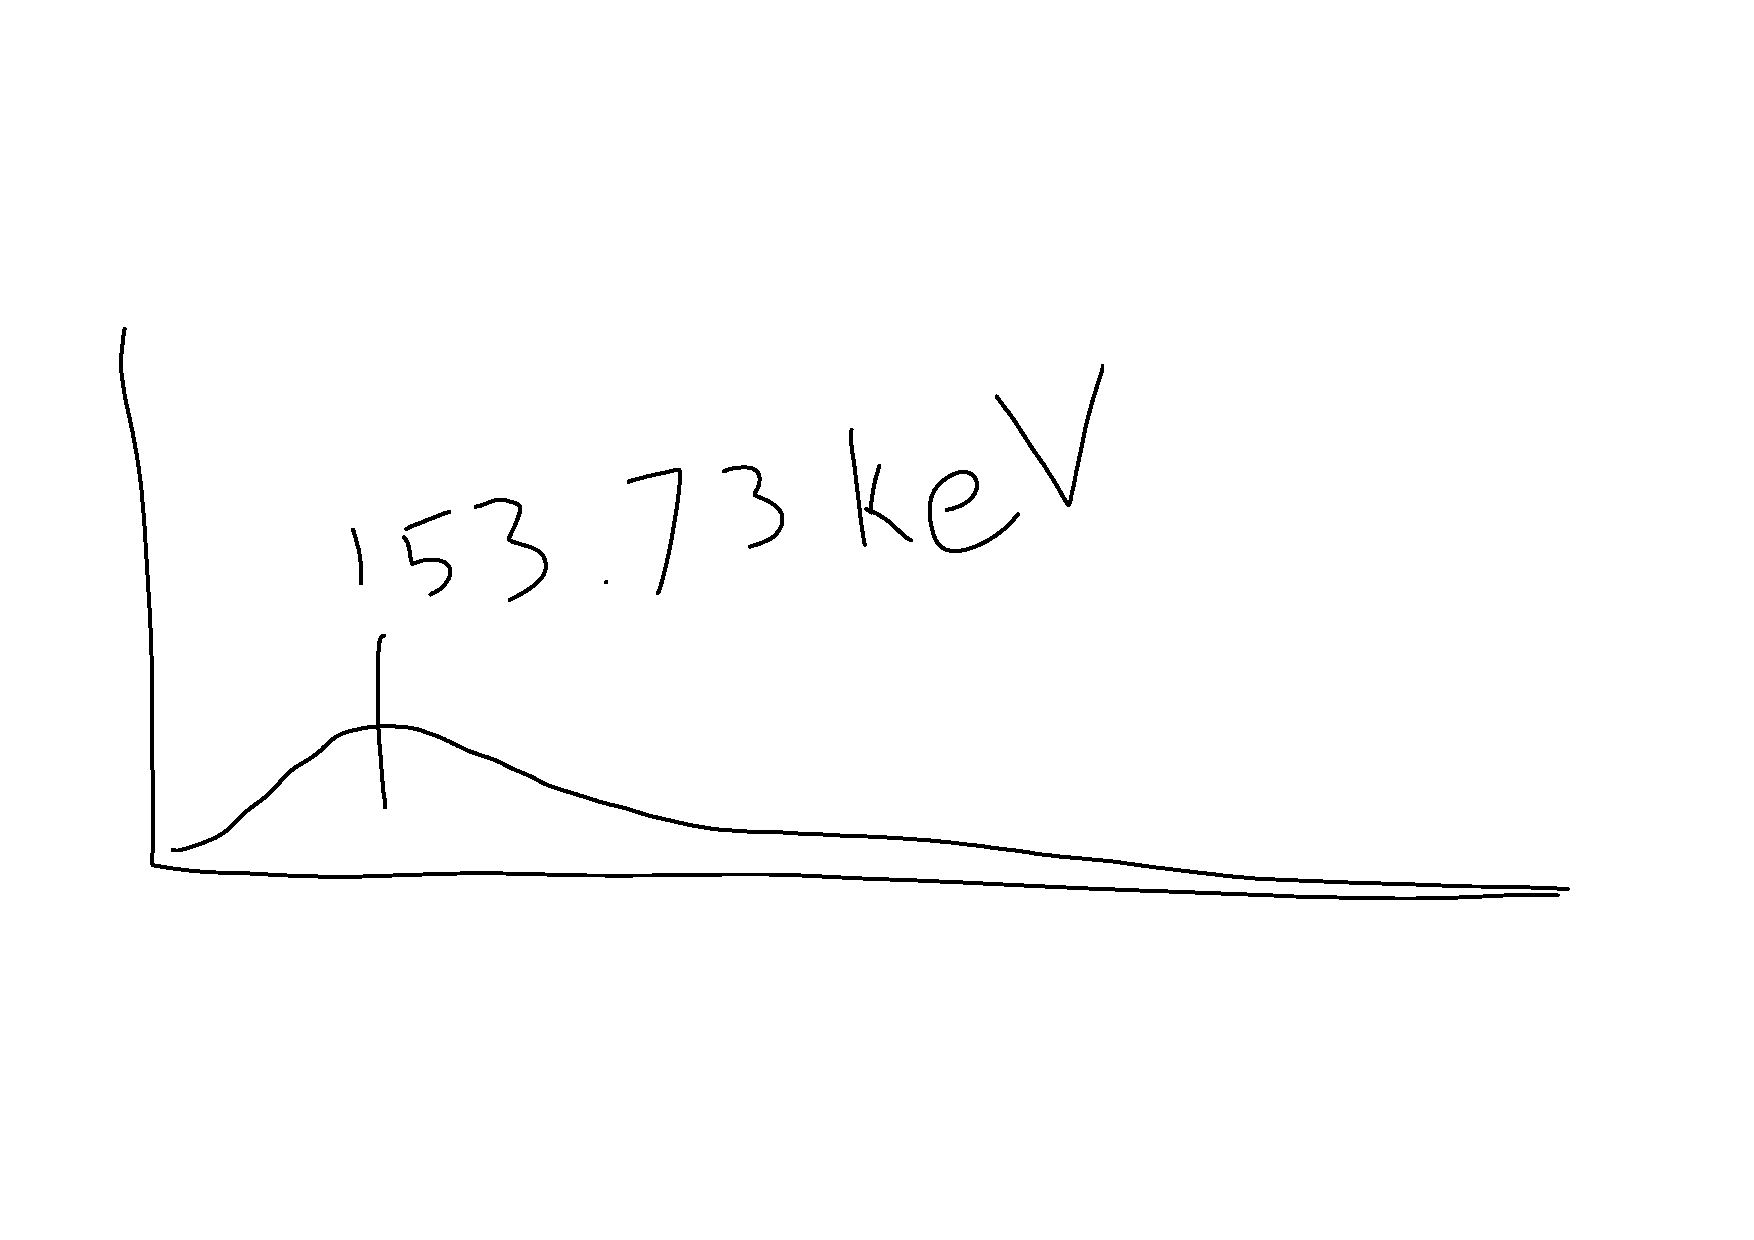
\includegraphics[width=0.75\textwidth]{figures/background_counts.pdf}
%     \caption{Background spectra of counts associated with varying energy bins. An elevated count level was identified at 153.73 keV}
% \end{figure}
\begin{itemize}
    \item with no sample, a background spectrum was recorded
    \item peak was 153.73 keV, FWHM was 1.04
    \item library suggested xenon 138
    \item \textbf{Data saved at: ./data/calibration\_spectrum\_bg.*}
\end{itemize}

\end{document}